\begin{frame}[standout]

    Bases de données document

\end{frame}

\begin{frame}{Caractéristiques des bases de données document}

    \begin{definitionbox}
        Dans une base de données orientée document, les données sont stockées sous forme de \textbf{documents} structurés, généralement au format \textbf{JSON}, \textbf{BSON}, ou \textbf{XML}.

        Chaque document représente un enregistrement, ce qui permet de stocker des données hiérarchiques et complexes.
    \end{definitionbox}

    \begin{noteblock}
        \begin{itemize}
            \item Très flexible : chaque document peut avoir une structure différente.
            \item Capable de stocker des données complexes et imbriquées.
        \end{itemize}
        $\hookrightarrow$ Idéal pour des applications nécessitant un modèle de données flexible et des mises à jour fréquentes.
    \end{noteblock}
\end{frame}

\begin{frame}{Bases de données document}
    \begin{figure}[htb]
        \centering
        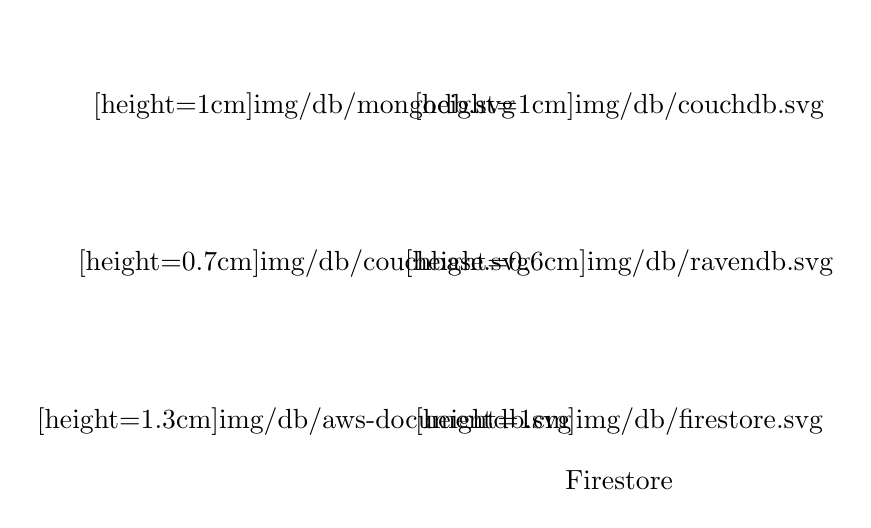
\begin{tikzpicture}
            \node[minimum width=3cm, minimum height=2cm] at (0, 0) {\includesvg[height=1cm]{img/db/mongodb.svg}};
            \node[minimum width=3cm, minimum height=2cm] at (4, 0) {\includesvg[height=1cm]{img/db/couchdb.svg}};
            \node[minimum width=3cm, minimum height=2cm] at (0, -2) {\includesvg[height=0.7cm]{img/db/couchbase.svg}};
            \node[minimum width=3cm, minimum height=2cm] at (4, -2) {\includesvg[height=0.6cm]{img/db/ravendb.svg}};
            \node[minimum width=3cm, minimum height=2cm] at (0, -4) {\includesvg[height=1.3cm]{img/db/aws-documentdb.svg}};
            \node[minimum width=3cm, minimum height=1cm,label=below:Firestore] at (4, -4) {\includesvg[height=1cm]{img/db/firestore.svg}};
        \end{tikzpicture}
    \end{figure}
\end{frame}

\begin{frame}[fragile]{Exemple de document JSON}

\begin{minted}[fontsize={\fontsize{6.7}{7.7}\selectfont}]{json}
[
    {
        "title": "Mamma Mia!",
        "year" : 2008,
        "cast" : {
            "director" : "Phyllida Lloyd",
            "actors" : ["Meryl Streep", "Pierce Brosnan","Amanda Seyfried"]
        },
        "rating" : 6.4,
        "plot" : "The story of a bride-to-be trying to find her real father told
using hit songs by the popular '70s group ABBA."
    },
    {
        "title": "Inception",
        "year" : 2010,
        "rating" : 8.8,
        "genres" : ["Action", "Adventure", "Sci-Fi"],
        "plot" : "A thief who steals corporate secrets through the use of dream-sharing
technology is given the inverse task of planting an idea into the mind of a CEO."
    }
]
\end{minted}

\end{frame}

\begin{frame}{Comment fonctionnent les bases de données document ?}

    \begin{figure}
        \centering
        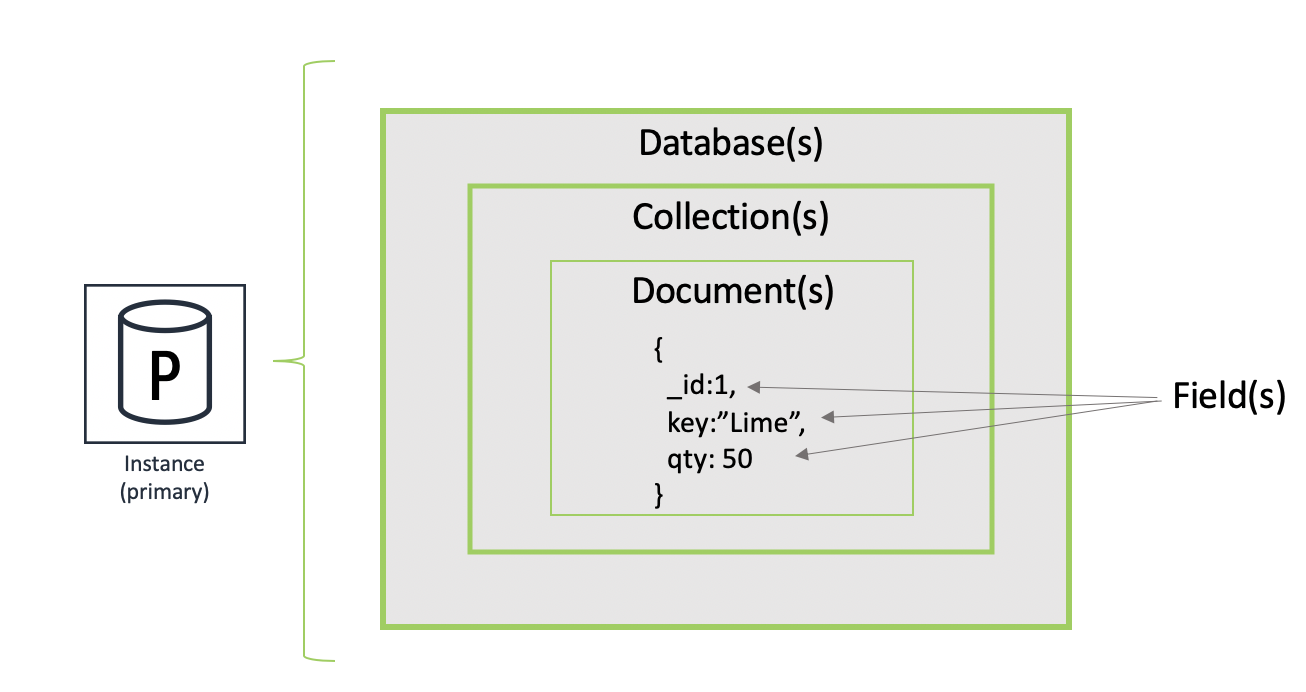
\includegraphics[width=0.8\textwidth]{img/json-document-database.png}
    \end{figure}

\end{frame}


\begin{frame}{Comment fonctionnent les bases de données document ?}

    \textbf{TODO : remplacer l'image par un filtrage sur les données de l'exemple JSON de l'exemple précédent.}

    \begin{figure}
        \centering
        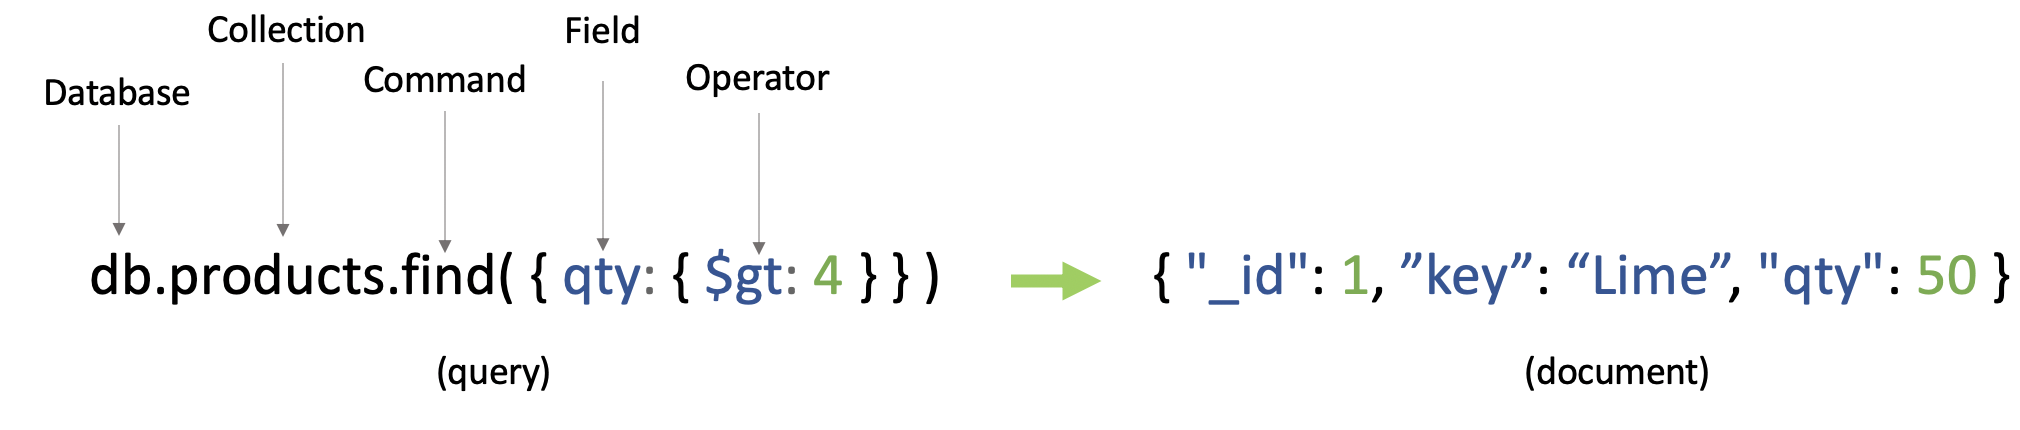
\includegraphics[width=0.8\textwidth]{img/json-database-query.png}
    \end{figure}

\end{frame}

\begin{frame}{Cas d'usages des bases de données document}

\begin{itemize}
    \item \textbf{Gestion du contenu sur les réseaux sociaux}\\
    $\hookrightarrow$ L'activité de chaque utilisateur est stockée sous forme d'un document contenant des informations imbriquées telles que les posts, commentaires, et connexions.
    \vspace{0.3cm}

    \item \textbf{Plateformes de gestion de contenu (CMS)}\\
    $\hookrightarrow$ Stockage de documents flexibles qui contiennent des informations sur des articles de blog, des images, des métadonnées, etc.
    \vspace{0.3cm}

    \item \textbf{Gestion des capteurs}\\
    $\hookrightarrow$ L'Internet des objets (IoT) permet de collecter un grand volume de données brutes à partir de capteurs (données non structurées et évolutives).
\end{itemize}
\end{frame}

% Gestion de contenu
% Une base de données document est un excellent choix pour les applications de gestion de contenu comme les blogs et les plateformes vidéo.
% Avec une base de données document, chaque entité que suit l'application peut être stockée comme un document unique.
% La base de données document est plus intuitive pour qu'un développeur puisse mettre à jour une application à mesure que les exigences évoluent.
% De plus, si le modèle de données doit être modifié, seuls les documents concernés doivent être mis à jour.
% Aucun schéma de mise à jour ou interruption de la base de données n'est nécessaire pour effectuer les modifications.

% Catalogues
% Les bases de données de documents sont un bon moyen de stocker des informations sur les catalogues.
% Par exemple, dans une application d'e-commerce, des produits différents ont souvent des attributs différents.
% Gérer des milliers d'attributs dans des bases de données relationnelles n'est pas efficace, et cela nuit aux performances de lecture.
% En utilisant une base de données document, les attributs de chaque produit peuvent être décrits dans un seul document pour une gestion aisée
% et une vitesse de lecture supérieure. Vous pouvez modifier les attributs d'un produit sans craindre de changer ceux d'un autre produit.

% Gestion des capteurs
% L'Internet des objets (IoT) permet aux entreprises de collecter régulièrement des données à partir d'appareils intelligents tels que des
% capteurs et des compteurs. Les données des capteurs arrivent généralement sous la forme d'un flux continu de valeurs variables.
% En raison de problèmes de latence, certains objets de données peuvent être incomplets, dupliqués ou manquants.
% En outre, vous devez collecter un volume important de données avant de pouvoir les filtrer ou les résumer à des fins d'analyse.
% Les magasins de documents sont plus pratiques dans ce cas. Vous pouvez rapidement stocker les données des capteurs telles quelles,
% sans avoir à les nettoyer ou à les rendre conformes à des schémas prédéterminés. Vous pouvez également les mettre à l'échelle selon vos
% besoins et supprimer des documents entiers une fois les analyses effectuées.

\begin{frame}{Avantages et inconvénients des bases de données document}
\vfill
\prosbox{
    \textbf{Avantages}
    \begin{itemize}
        \item Grande flexibilité dans le schéma, chaque document peut avoir une structure différente.
        \item Bonne gestion des données hiérarchiques ou imbriquées.
        \item Scalabilité horizontale facile grâce à la partition des documents.
    \end{itemize}
}
\vfill
\pause
\consbox{
    \textbf{Inconvénients}
    \begin{itemize}
        \item Performances limitées pour des requêtes complexes ou des jointures entre documents.
        \item Les mises à jour simultanées de documents imbriqués peuvent être plus complexes à gérer.
    \end{itemize}
}
\vfill
\end{frame}

\subsection{Flexibilité du schéma}

\begin{frame}{Quelle flexibilité de schéma ?}

    \begin{figure}[htb]
        \centering
        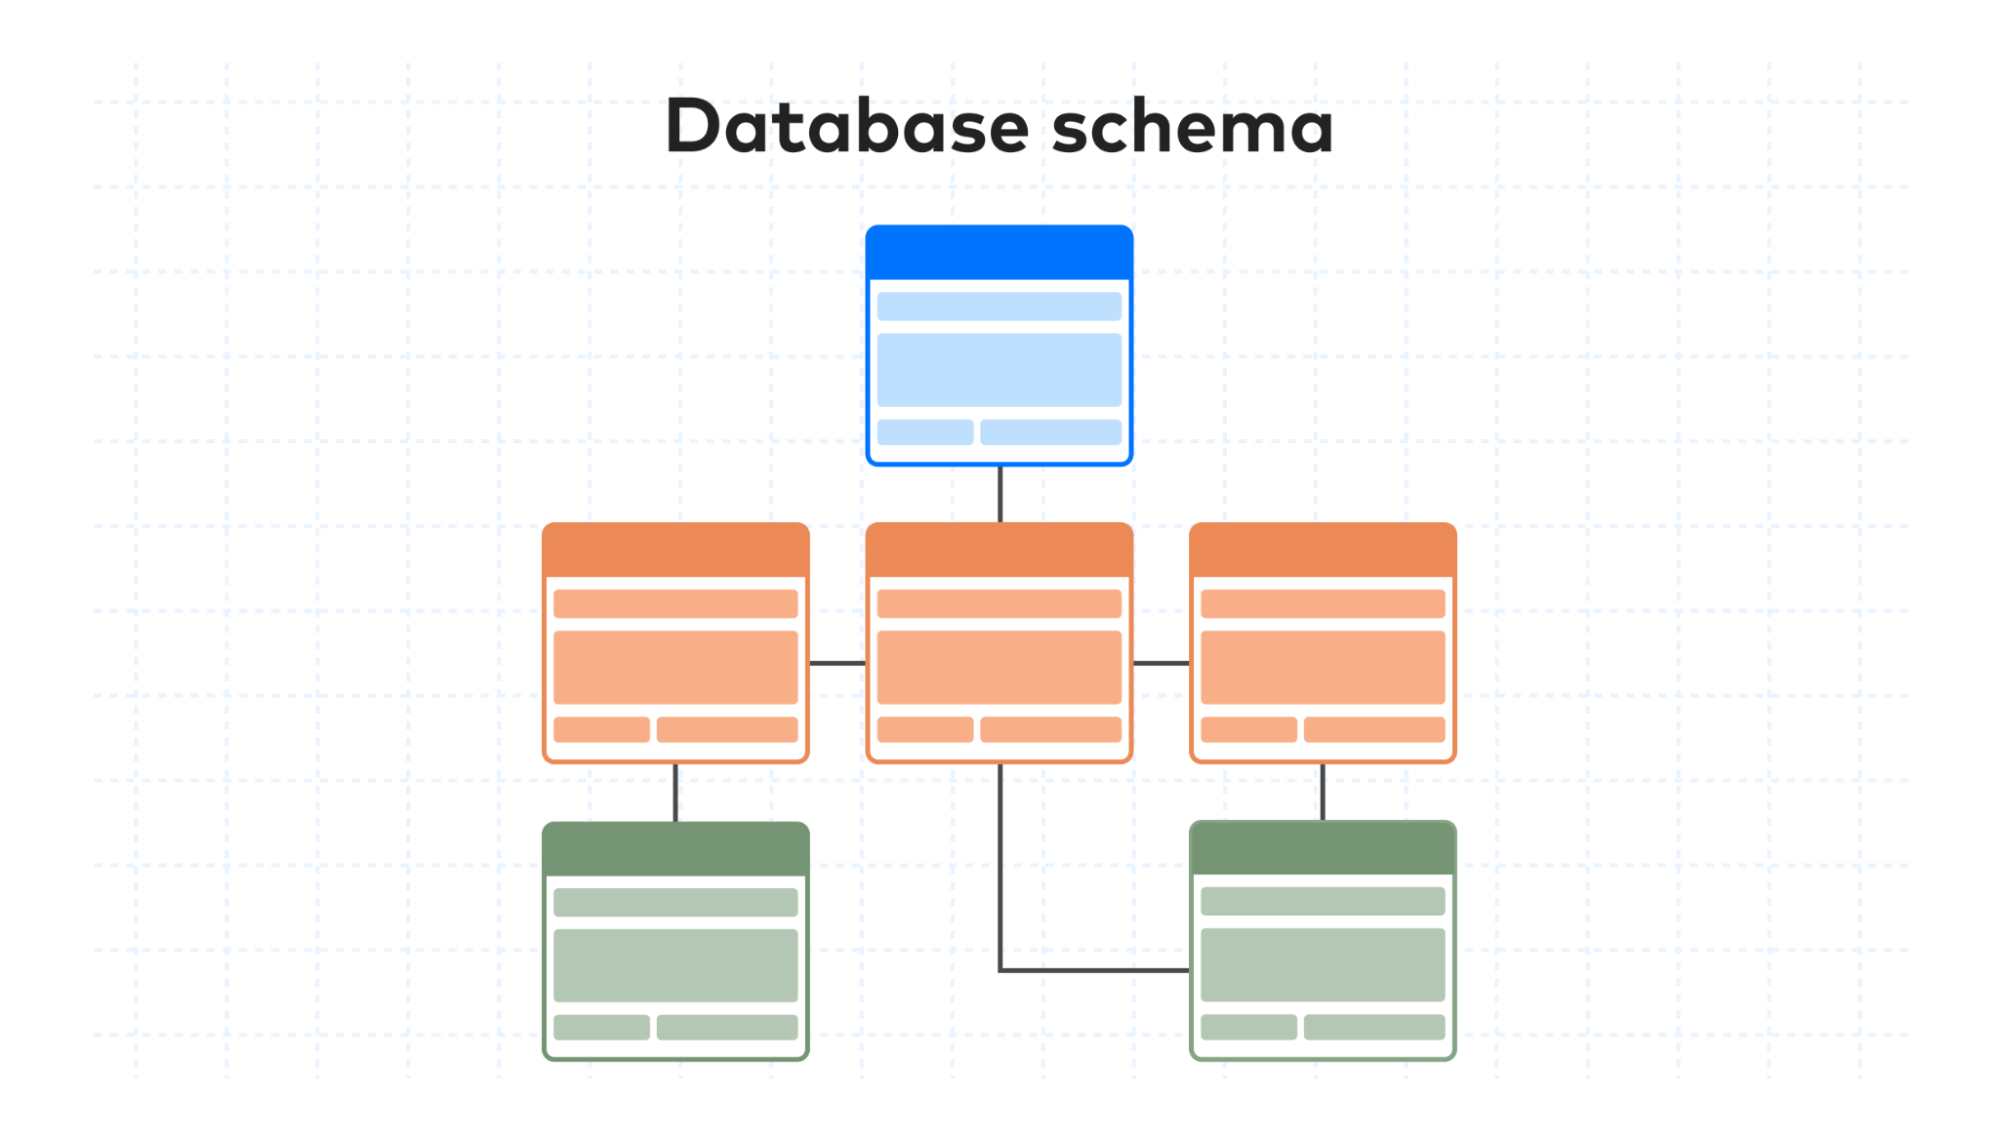
\includegraphics[width=0.9\textwidth]{img/database-schema.png}
    \end{figure}

\end{frame}


\begin{frame}{Schéma flexible}

    Donner example de schéma flexible

\end{frame}


\begin{frame}{Focus sur MongoDB}

\end{frame}

\begin{frame}{Étude de cas}

    Uber et MongoDB (gestion des trajets en temps réel).

    Problématique.
    Solution NoSQL choisie.
    Architecture mise en place.
    Résultats (performances, coûts).

\end{frame}
